\documentclass{beamer}
\usetheme{Hannover}
\setbeamersize{sidebar width left=0pt}
\usepackage[T1, T2A]{fontenc}
\usepackage[utf8]{inputenc}
\usepackage[russian]{babel}
\usepackage{hyperref}
\usepackage{graphicx}
\graphicspath{ {../Images/} }

\author{Григорий Матюхин}
\date{\today}
\title{Лабораторная работа \textnumero10.}
\subtitle{Основы работы с модулями ядра операционной системы}

\begin{document}
\begin{frame}[plain]
	\titlepage
\end{frame}
\section{Цель работы}
\begin{frame}[plain]
	\frametitle{Цель работы}
	Получить навыки работы с утилитами управления модулями ядра операционной системы.
\end{frame}

\subsection{Управление модулями ядра из командной строки}
\begin{itemize}
	\begin{frame}[plain]
		\frametitle{Управление модулями ядра из командной строки}
		\item Посмотрите, какие устройства имеются в вашей системе и какие модули ядра с ними связаны:
		\\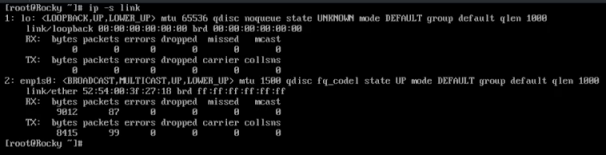
\includegraphics{1.png}
	\end{frame}
	\begin{frame}[plain]
		\item Посмотрите, какие модули ядра загружены:
		\\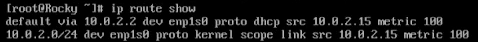
\includegraphics{2.png}
	\end{frame}
	\begin{frame}[plain]
		\item Посмотрите, загружен ли модуль \texttt{ext4}:
		\\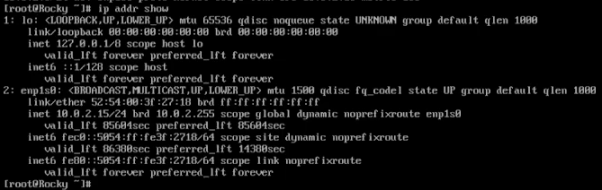
\includegraphics{3.png}
	\end{frame}
	\begin{frame}[plain]
		\item Загрузите модуль ядра \texttt{ext4}. Убедитесь, что модуль загружен, посмотрев список загруженных модулей:
		\\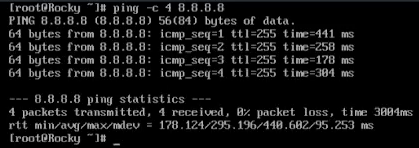
\includegraphics{4.png}
	\end{frame}
	\begin{frame}[plain]
		\item Посмотрите информацию о модуле ядра \texttt{ext4}:
		\\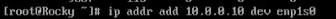
\includegraphics{5.png}
	\end{frame}
	\begin{frame}[plain]
		\item Попробуйте выгрузить модуль ядра \texttt{ext4}:
		\\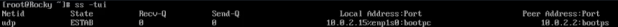
\includegraphics{6.png}
	\end{frame}
	\begin{frame}[plain]
		\item Попробуйте выгрузить модуль ядра \texttt{xfs}:
		\\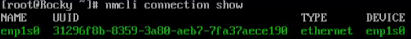
\includegraphics{7.png}
	\end{frame}
\end{itemize}

\subsection{Загрузка модулей ядра с параметрами}
\begin{itemize}
	\begin{frame}[plain]
		\frametitle{Загрузка модулей ядра с параметрами}
		\item Посмотрите, загружен ли модуль \texttt{bluetooth}:
		\item Загрузите модуль ядра \texttt{bluetooth}:
		\\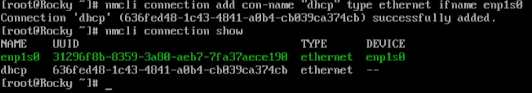
\includegraphics{8.png}
	\end{frame}
	\begin{frame}[plain]
		\item Посмотрите список модулей ядра, отвечающих за работу с \texttt{bluetooth}:
		\\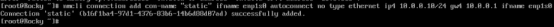
\includegraphics{9.png}
	\end{frame}
	\begin{frame}[plain]
		\item Посмотрите информацию о модуле \texttt{bluetooth}:
		\\
\includegraphics{10.png}
	\end{frame}
	\begin{frame}[plain]
		\item Выгрузите модуль ядра \texttt{bluetooth}:
		\\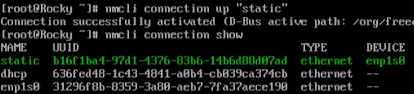
\includegraphics{11.png}
	\end{frame}
\end{itemize}

\subsection{Обновление ядра системы}
\begin{itemize}
	\begin{frame}[plain]
		\frametitle{Обновление ядра системы}
		\item Посмотрите версию ядра, используемую в операционной системе:
		\\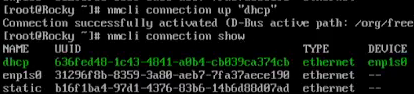
\includegraphics{12.png}
	\end{frame}
	\begin{frame}[plain]
		\item Выведите на экран список пакетов, относящихся к ядру операционной системы:
		\\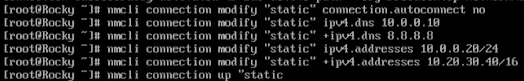
\includegraphics{13.png}
	\end{frame}
	\begin{frame}[plain]
		\item Обновите систему, чтобы убедиться, что все существующие пакеты обновлены, так как это важно при установке/обновлении ядер \texttt{Linux} и избежания конфликтов:
		\\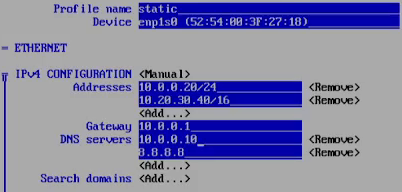
\includegraphics{14.png}
	\end{frame}
	\begin{frame}[plain]
		\item Обновите ядро операционной системы, а затем саму операционную систему:
		\\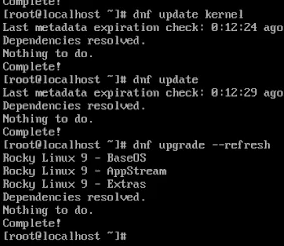
\includegraphics{15.png}
	\end{frame}
	\begin{frame}[plain]
		\item Перегрузите систему. При загрузке выберите новое ядро.
		\\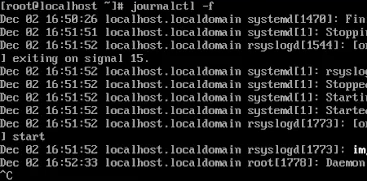
\includegraphics{16.png}
	\end{frame}
	\begin{frame}[plain]
		\item Посмотрите версию ядра, используемую в операционной системы:
		\\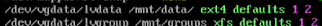
\includegraphics{17.png}
	\end{frame}
\end{itemize}

\section{Вывод}
\begin{frame}[plain]
	\frametitle{Вывод}
	В ходе выполнения данной работы я получил навыки работы с утилитами управления модулями ядра операционной системы.
\end{frame}

\end{document}
